\documentclass[10pt]{article}
\usepackage[a4paper,margin=0.82in]{geometry}
\usepackage{amsmath,amssymb}
\usepackage{graphicx}
\usepackage{booktabs,tabularx,array}
\usepackage{caption}
\usepackage{subcaption}
\usepackage{float}
\usepackage{enumitem}
\usepackage{xcolor}
\usepackage{microtype}
\usepackage{hyperref}
\hypersetup{colorlinks=true,linkcolor=blue,citecolor=blue,urlcolor=blue}
\newcommand{\mmals}{\textsc{MMALS}}
\newcommand{\rc}{\textsc{RC2O}}
\title{\textbf{Stable-Plastic Context Memory for Dataset-Agnostic Continual Routing in MMALS}\\
\large A Backward-Compatible Architectural Proposal and Reviewer-Facing Evaluation Protocol}
\author{Guillaume Harbonnier\\MMALS Research Program}
\date{Design note: June 12, 2026}
\begin{document}
\maketitle

\begin{abstract}
The latest \textsc{CORe50} experiments expose a structural mismatch in the current \mmals{} context path. A v2.3 rescue ablation improves average accuracy, forgetting, class coverage and host diversity, yet fails to recover the two oldest contexts. The isolated exponential-moving-average intervention also fails. Inspection shows that the retention objective directly trains a single-input context encoder, whereas the deployed posterior is dominated by prototype evidence. This note proposes a dataset-agnostic stable-plastic context-memory module that trains the posterior actually used at inference, preserves slow context anchors while allowing plastic updates, and provides an exact \texttt{legacy} operating mode for reproducing all prior notebooks. The module is designed to work after any input representation, including raw-flat MNIST-family inputs and frozen visual features for SplitCIFAR or CORe50. The proposal includes three backward-compatible modes, stable and plastic memory banks, adaptive fusion, teacher-posterior and functional distillation, overlap-aware soft targets, a confident-collapse veto, computational controls, an ablation matrix, falsification criteria and cross-dataset regression gates. This is an architectural proposal and test plan, not evidence that the redesign already improves performance.
\end{abstract}

\section{Reviewer-facing motivation}
The proposal is driven by a falsified hypothesis rather than by architecture inflation. In the two-seed CORe50 v2.3 ablation, the combined rescue raises final average accuracy from $0.2734$ to $0.3171$, minimum-task accuracy from $0.0050$ to $0.0513$, reduces mean zero-recall classes from $9.0$ to $0.5$, and increases effective hosts from about $2.04$ to $8.68$. Nevertheless, oldest-two context top-1 remains $0.0$. The isolated context EMA intervention reduces oldest-two task accuracy and increases zero-recall classes. Therefore, simply preserving prototypes more strongly is not sufficient.

The relevant mismatch is:
\begin{equation}
\text{training objective} \longrightarrow q_{\mathrm{single}},
\qquad
\text{deployed decision} \longrightarrow q_{\mathrm{prototype}} \text{ dominated}.
\end{equation}
When the loss optimizes a weakly weighted branch and the dominant inference branch is only indirectly affected, the system can report improved intermediate-context behavior while the oldest contexts remain unrecovered.

This note asks a narrow question:
\begin{quote}
Can a common context-memory layer preserve old contextual evidence, remain plastic under drift, support legitimate ambiguity, and reproduce historical results exactly when disabled?
\end{quote}

\section{Design requirements}
A reviewer should be able to reject the module if any of the following requirements are not met.
\begin{enumerate}[leftmargin=*]
\item \textbf{Dataset agnosticism.} No branch may depend on dataset names, fixed class IDs, ``old tasks 0 and 1,'' or a fixed number of contexts or hosts.
\item \textbf{Backward compatibility.} A \texttt{legacy} mode must reproduce the historical deployed posterior and permit old checkpoints to be evaluated without recovering every historical notebook.
\item \textbf{Deployed-posterior training.} Retention losses must act on the posterior used during inference, not only on a subordinate component.
\item \textbf{Stable-plastic separation.} Slow anchors and rapidly updated prototypes must be explicit, separately audited objects.
\item \textbf{Ambiguity preservation.} Overlapping contexts must support soft targets and guarded mixed-context routing.
\item \textbf{Bounded complexity.} The module should add modest state and computation relative to the existing router, with exact cost reporting.
\item \textbf{No test leakage.} Fusion calibration, repair and selection must use train, repair or policy-validation memory only.
\end{enumerate}

\begin{figure}[H]
\centering
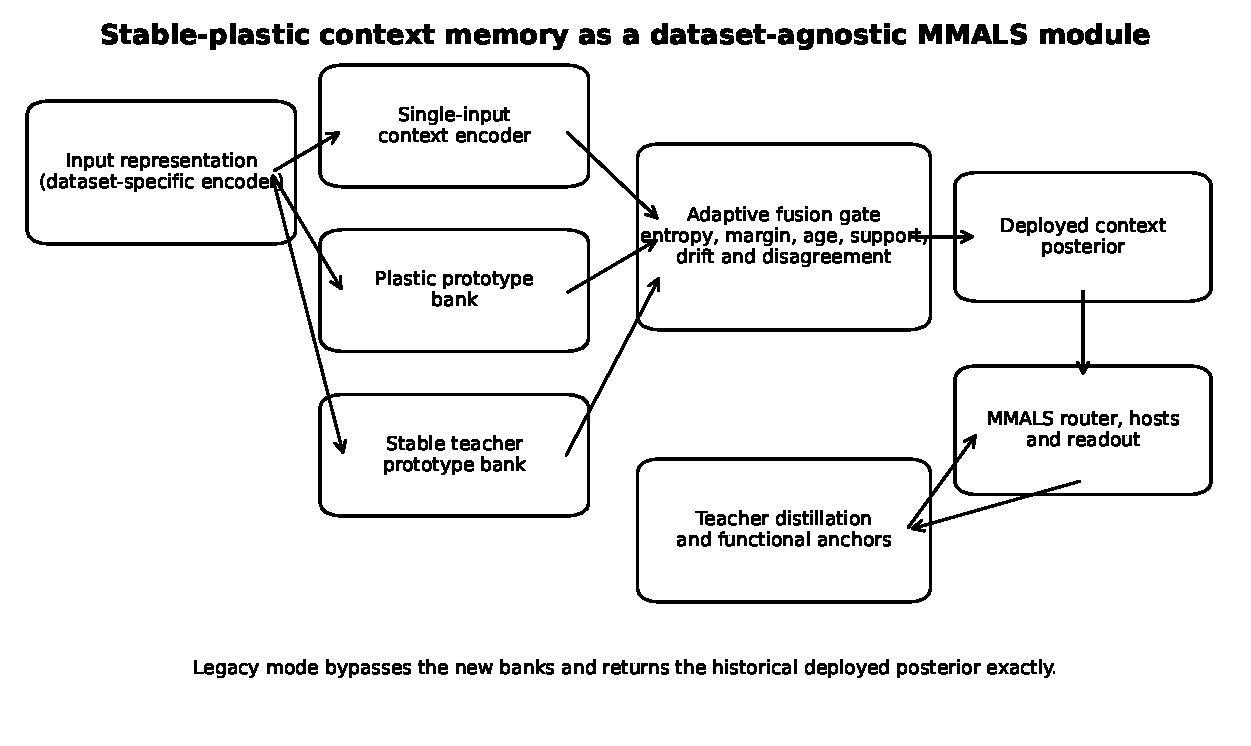
\includegraphics[width=0.95\linewidth]{figures/stable_plastic_architecture.pdf}
\caption{Proposed dataset-agnostic context-memory module. The input encoder remains dataset-specific; the context-memory interface is common.}
\end{figure}

\section{Backward-compatible operating modes}
The module must expose an explicit mode contract rather than silently changing the behavior of \mmals{}.

\begin{table}[H]
\centering
\caption{Operating modes and guarantees.}
\begin{tabularx}{\linewidth}{@{}l p{0.22\linewidth} X X@{}}
\toprule
Mode & Purpose & Context posterior & Required guarantee \\
\midrule
\texttt{legacy} & Exact historical reproduction & Existing single/prototype posterior and fixed blend & Bitwise or tolerance-bounded equivalence on stored checkpoints and test fixtures. \\
\texttt{stable\_plastic} & Controlled architectural ablation & Single encoder plus stable and plastic prototype banks under fixed fusion & No dataset-specific branches; all weights and updates exported. \\
\texttt{adaptive} & Proposed deployable mode & Validation-calibrated fusion with disagreement and confident-collapse veto & Regression gates on MNIST family and SplitCIFAR10 before promotion. \\
\bottomrule
\end{tabularx}

\end{table}

\begin{figure}[H]
\centering
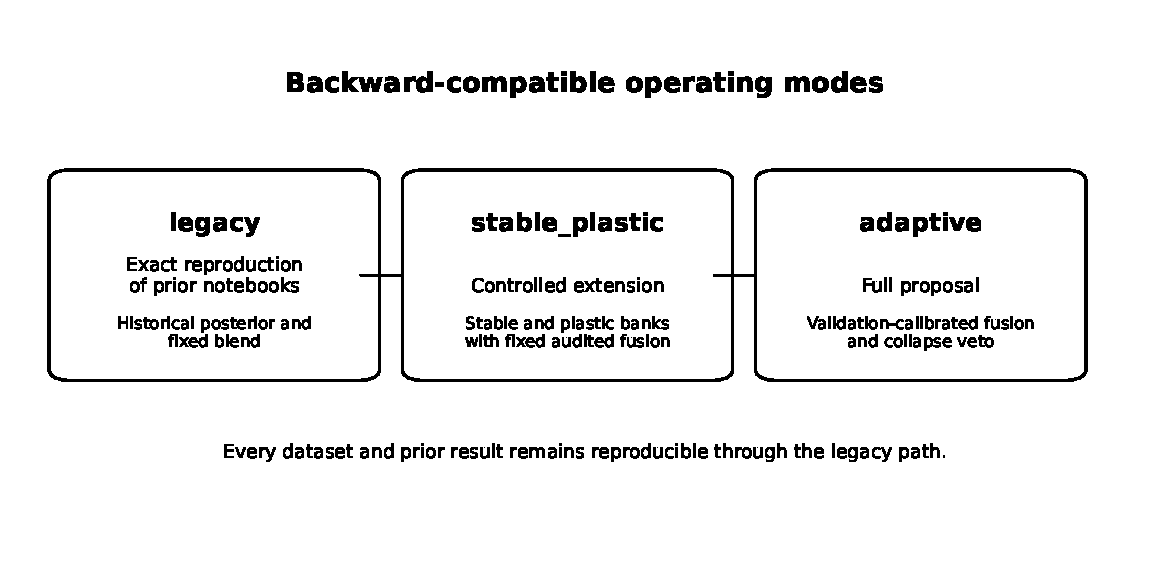
\includegraphics[width=0.86\linewidth]{figures/operating_modes.pdf}
\caption{The proposal is an extension of the existing context path, not an irreversible fork.}
\end{figure}

In \texttt{legacy} mode, the module must implement
\begin{equation}
q_{\mathrm{deploy}}^{\mathrm{new}}(c\mid x,m)
=
q_{\mathrm{deploy}}^{\mathrm{historical}}(c\mid x,m)
\end{equation}
within a declared numerical tolerance. The release package includes a reference module and tests for this contract.

\section{Stable and plastic memory banks}
For each context $c$, the module maintains two memory states.

The \emph{plastic} prototype $P_c^{(t)}$ follows current repair memory and recent observations:
\begin{equation}
P_c^{(t)} \leftarrow (1-\eta_p)P_c^{(t-1)} + \eta_p\,\widehat{P}_c^{(t)},
\end{equation}
where $\eta_p$ may be relatively large.

The \emph{stable} anchor $S_c^{(t)}$ changes slowly and only when support and validation evidence are sufficient:
\begin{equation}
S_c^{(t)} \leftarrow (1-\eta_s)S_c^{(t-1)} + \eta_s\,\widehat{S}_c^{(t)},
\qquad \eta_s \ll \eta_p.
\end{equation}

Each bank records support count, age, last update, dispersion and drift. Stable memory is not ``frozen forever.'' It is slow, evidence-gated memory. Plastic memory is not trusted by default; it provides adaptation evidence.

For a sample representation $e$ and mediated latent $z$, the module computes branch posteriors
\begin{equation}
q_s(c\mid e,z), \qquad q_p(c\mid e,z), \qquad q_0(c\mid e),
\end{equation}
for stable, plastic and single-input evidence respectively.

\section{Adaptive fusion}
The proposed deployed posterior is
\begin{equation}
q_{\mathrm{deploy}}(c\mid x,m)
=
\alpha_0 q_0(c\mid e)
+
\alpha_p q_p(c\mid e,z)
+
\alpha_s q_s(c\mid e,z),
\end{equation}
where $\alpha_0+\alpha_p+\alpha_s=1$ and $\alpha_i\geq0$.

The fusion weights are functions of auditable features:
\begin{equation}
\boldsymbol{\alpha}=g( H(q_0),H(q_p),H(q_s),\Delta_{sp},\gamma, a, n, d),
\end{equation}
where $H$ is entropy, $\Delta_{sp}$ is stable-plastic disagreement, $\gamma$ is the top-two margin, $a$ is context age, $n$ is support and $d$ is drift. The first implementation should support both a rule-based gate and a small learned gate. The rule-based gate is preferred for the first causal ablation because its decisions are easier to audit.

The adaptive mode must permit three limiting cases:
\begin{align}
\boldsymbol{\alpha}&=(1,0,0) && \text{single-input fallback},\\
\boldsymbol{\alpha}&=(0,1,0) && \text{plastic adaptation},\\
\boldsymbol{\alpha}&=(0,0,1) && \text{stable-anchor protection}.
\end{align}
It must also permit the exact historical blend in \texttt{legacy} mode.

\section{Train the posterior used at inference}
For replayed old-context samples $(x,c)$, the first retention term is direct cross-entropy on the deployed posterior:
\begin{equation}
\mathcal{L}_{\mathrm{ctx}}=
-\log q_{\mathrm{deploy}}(c\mid x,m).
\end{equation}

A teacher snapshot from the previous checkpoint provides a soft retention target:
\begin{equation}
\mathcal{L}_{\mathrm{ctxKD}}
=
T^2 D_{\mathrm{KL}}\left(
q^{\star}_{\mathrm{deploy}}(\cdot\mid x,m;T)
\parallel
q_{\mathrm{deploy}}(\cdot\mid x,m;T)
\right).
\end{equation}
This term preserves uncertainty where uncertainty was previously legitimate. It does not force a hard context label when the teacher distribution was mixed.

\section{Functional preservation beyond context labels}
Correct context identity is useful but insufficient. The CORe50 oracle gap shows that even perfect context would leave substantial classification error. The old-state objective should therefore preserve a compact functional bundle:
\begin{equation}
\mathcal{L}_{\mathrm{old}}
=
\lambda_c\mathcal{L}_{\mathrm{ctxKD}}
+
\lambda_r\lVert r-r^{\star}\rVert_2^2
+
\lambda_z\lVert z_f-z_f^{\star}\rVert_2^2
+
\lambda_y T_y^2D_{\mathrm{KL}}(p^{\star}_y\parallel p_y).
\end{equation}
This formulation follows the earlier \mmals{} finding that route preservation alone is not equivalent to preservation of the mediated latent function.

To limit memory cost, teacher bundles can be stored for a small balanced replay subset or reconstructed from periodic checkpoint anchors. The implementation must report bytes per context and bytes per replay item.

\section{Overlap-aware targets}
The MNIST-family overlap chain contains legitimate ambiguity. For example, a shared class may support two adjacent contexts. A hard one-hot context target can therefore destroy a useful mixed posterior.

For overlapping contexts, the target can be a normalized support distribution
\begin{equation}
q^{\star}(c\mid x)
\propto
\mathbf{1}[c\in\mathcal{C}(y)]\,w_c(x),
\end{equation}
where $\mathcal{C}(y)$ is the set of contexts containing class $y$ and $w_c$ may use teacher evidence or prototype distance. This is a protocol option derived from task metadata, not a dataset-name condition.

\begin{table}[H]
\centering
\caption{Compatibility implications across current benchmark families.}
\begin{tabularx}{\linewidth}{@{}l p{0.24\linewidth} X@{}}
\toprule
Dataset family & Context structure & Design consequence \\
\midrule
MNIST / FashionMNIST overlap chain & Adjacent tasks share classes and ambiguity is legitimate. & Use soft teacher targets and permit guarded mixed-context posteriors; do not force hard prototype separation. \\
Rotated / Permuted MNIST & Contexts reflect transformation or domain changes. & Stable anchors preserve transformation identity while the plastic bank adapts to drift. \\
SplitCIFAR10 & Five disjoint class groups with a strong current result. & New module must be opt-in and pass strict non-regression gates before becoming default. \\
SplitCIFAR100 & Ten large class groups with representation/readout limits. & Context redesign may help retention but cannot substitute for stronger representation and readout controls. \\
CORe50 & Ten object groups with observed recency and host collapse. & Primary failure-driven test bed for stable-plastic memory and deployed-posterior distillation. \\
\bottomrule
\end{tabularx}

\end{table}

\section{Confident-collapse veto}
The CORe50 failure was not merely high entropy. Old samples were sometimes mapped to a recent context with near-zero entropy. Therefore, low entropy cannot be interpreted as correctness.

Define the predicted context age gap $\Delta a=a(\hat{c})-a(c_s)$, where $c_s$ is the stable-anchor winner. A confident recent-context collapse alert is triggered when
\begin{equation}
H(q_{\mathrm{deploy}})<h_{\min},\qquad
\Delta a>a_{\max},\qquad
q_s(c_s)-q_s(\hat{c})>\delta_s.
\end{equation}
The response is not always to force $c_s$. Depending on validation configuration, the module may:
\begin{enumerate}[leftmargin=*]
\item increase stable-anchor weight;
\item use a guarded mixture of the stable and single branches;
\item route through multiple contexts;
\item abstain to a safe policy family.
\end{enumerate}
Every intervention must be exported with reason codes.

\section{Dataset-agnostic interface}
The module operates after the input representation. Its required dimensions derive from configuration:
\begin{equation}
N_{\mathrm{contexts}},\quad d_e,\quad d_z,\quad N_{\mathrm{hosts}},\quad \text{support metadata}.
\end{equation}
It must not inspect dataset names or class literals. The same interface applies to raw-flat MNIST inputs, frozen CNN features, future graph encoders or other representations.

A minimal forward contract is:
\begin{verbatim}
posterior, audit = context_memory(
    q_single=q_single,
    stable_logits=stable_logits,
    plastic_logits=plastic_logits,
    metadata={entropy, margin, age, support, drift, disagreement},
    mode="legacy|stable_plastic|adaptive",
)
\end{verbatim}
The returned audit object includes fusion weights, branch winners, disagreement, collapse-veto status and fallback reason.

\section{Computational and memory cost}
For $C$ contexts and prototype dimension $d$, two prototype banks add approximately $2Cd$ floating-point values plus metadata. With $C=10$ and $d=256$, this is negligible relative to the host backbone. The learned adaptive gate should remain small, for example a two-layer MLP over branch diagnostics, not over raw images.

The expensive part is functional teacher memory. The first implementation should compare:
\begin{enumerate}[leftmargin=*]
\item posterior-only distillation;
\item posterior plus route anchors;
\item posterior, route and latent anchors;
\item full output distillation.
\end{enumerate}
The smallest variant passing retention gates should be preferred.

\section{Ablation matrix}
The redesign must not be evaluated only as one combined ``full rescue.'' Each hypothesis is isolated.

\begin{table}[H]
\centering
\caption{Required mechanism ablations.}
\begin{tabularx}{\linewidth}{@{}l X l@{}}
\toprule
Variant & Isolated question & Promotion role \\
\midrule
\texttt{legacy} & Can previous results be reproduced without old notebooks? & Mandatory reference \\
\texttt{current\_ema} & Does the v2.3 EMA intervention reproduce its observed failure? & Failure control \\
\texttt{adaptive\_blend\_only} & Was fixed prototype dominance the main mismatch? & Mechanism isolation \\
\texttt{stable\_plastic\_only} & Do slow anchors prevent prototype drift? & Mechanism isolation \\
\texttt{deployed\_posterior\_distill} & Does training the actual inference posterior retain old contexts? & Mechanism isolation \\
\texttt{stable\_plastic\_plus\_distill} & Do the two corrections interact positively? & Candidate module \\
\texttt{oracle\_blend\_diagnostic} & What is the achievable context ceiling without deployment leakage? & Diagnostic only \\
\bottomrule
\end{tabularx}

\end{table}

Each branch must export separate top-1 accuracy, entropy and confusion for
\begin{equation}
q_0,\quad q_{\mathrm{feature}},\quad q_{\mathrm{latent}},\quad q_p,\quad q_s,\quad q_{\mathrm{deploy}}.
\end{equation}
Results must also be grouped by context age: oldest two, early-middle, late-middle and newest two.

\section{Promotion and regression gates}
\begin{table}[H]
\centering
\caption{Initial promotion gates. Thresholds are preregistered engineering gates, not universal constants.}
\begin{tabular}{@{}lr@{}}
\toprule
Gate & Required value \\
\midrule
Oldest-two context top-1 gain & $\geq +0.20$ \\
Oldest-two task accuracy gain & $\geq +0.03$ \\
Zero-recall class reduction & $\geq 2$ \\
Final average accuracy regression & $\leq 0.02$ \\
Recent-two task regression & $\leq 0.03$ \\
Confident recent-context collapse & Strongly reduced \\
SplitCIFAR10 final accuracy regression & $\leq 0.01$ \\
\bottomrule
\end{tabular}

\end{table}

The first mechanism test remains CORe50 seeds 0 and 4. If the candidate passes, it proceeds through the regression chain shown below.

\begin{figure}[H]
\centering
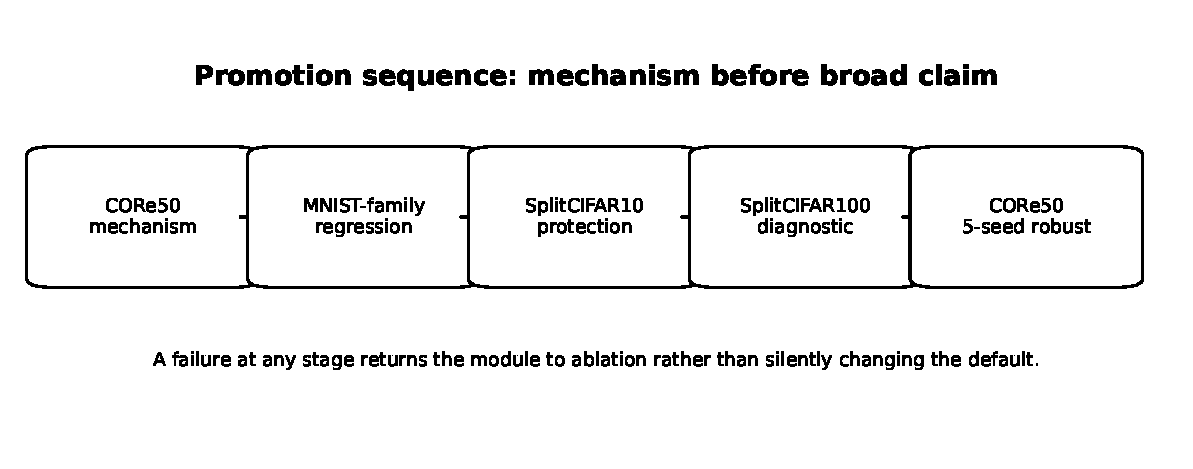
\includegraphics[width=0.92\linewidth]{figures/evaluation_roadmap.pdf}
\caption{Cross-dataset promotion sequence. The qualified SplitCIFAR10 result is protected before the redesign becomes a default backbone component.}
\end{figure}

MNIST-family regression must preserve qualitative selector behavior: clean MNIST should not be over-guarded, FashionMNIST ambiguity should remain protected, PermutedMNIST should retain simple/global options, and RotatedMNIST should retain weak-boundary calibration when validation evidence supports it.

\section{Reviewer questions and planned answers}
\subsection*{Is the proposal merely more capacity?}
No claim will be accepted without parameter, memory and latency deltas. The key mechanism variants share the same host backbone. Legacy, fixed stable-plastic and adaptive fusion are compared at matched representation and host count before integration with larger features or additional hosts.

\subsection*{Does the stable bank just freeze old tasks?}
No. Stable anchors are slowly updated and evidence-gated. The module permits shared contexts and soft targets. The ablation compares frozen, slow and plastic updates.

\subsection*{Could the module overfit CORe50?}
The interface contains no CORe50 literals. Promotion requires MNIST-family and SplitCIFAR10 regression. SplitCIFAR100 is used as a harder diagnostic before returning to five-seed CORe50 evidence.

\subsection*{Does teacher distillation prevent learning new contexts?}
Plasticity is measured explicitly through newest-task and recent-two-task accuracy. A candidate fails if recent performance regresses beyond the preregistered bound.

\subsection*{Can previous results still be reproduced?}
Yes, only if legacy-equivalence tests pass. Historical checkpoints should load through a versioned adapter that reconstructs missing stable/plastic state as disabled tensors and returns the original posterior.

\subsection*{Does the proposal prove backward transfer?}
No. The intended claims are retention, context stability, reduced collapse and bounded plasticity loss. Positive backward transfer remains a separate hypothesis.

\section{Falsification criteria}
The redesign should be rejected or delayed if:
\begin{enumerate}[leftmargin=*]
\item it fails to raise oldest-context accuracy on seeds 0 and 4;
\item gains disappear when representation and host count are matched;
\item legacy mode cannot reproduce stored outputs;
\item MNIST-family ambiguity is harmed by hard context separation;
\item SplitCIFAR10 regresses beyond the declared limits;
\item improvements require disproportionate memory or inference latency;
\item the adaptive gate becomes a non-auditable dataset classifier;
\item the module improves context top-1 but not old-task or class retention.
\end{enumerate}

\section{Implementation and release contract}
A versioned checkpoint should include:
\begin{itemize}[leftmargin=*]
\item context-memory schema version;
\item operating mode;
\item legacy blend parameters;
\item stable and plastic prototype banks;
\item support, age, dispersion and drift metadata;
\item fusion-gate state;
\item teacher-anchor configuration;
\item hash of the representation and router configuration.
\end{itemize}

The companion GitHub package includes a reference PyTorch module and unit tests for legacy equivalence, probability normalization, arbitrary context counts and absence of dataset-specific logic. The module is a design reference and is not yet integrated into the full training notebook.

\section{Conclusion}
The proposed stable-plastic module is a localized evolution of the \mmals{} backbone. It does not replace the hosts, transformations, mediated latent state, readout, audit layers or \rc{} policy framework. It replaces a fixed and partly mismatched context-memory interface with a versioned, backward-compatible component that separates slow and fast memory, trains the deployed posterior, preserves legitimate ambiguity and exposes its decisions. The proposal is justified by a concrete failed promotion gate and is accompanied by a sequence that can disprove it before any broad claim is made.

\begin{thebibliography}{10}
\bibitem{parisi2019} G. I. Parisi, R. Kemker, J. L. Part, C. Kanan, and S. Wermter. Continual lifelong learning with neural networks: A review. \emph{Neural Networks}, 113:54--71, 2019.
\bibitem{kirkpatrick2017} J. Kirkpatrick et al. Overcoming catastrophic forgetting in neural networks. \emph{PNAS}, 114(13):3521--3526, 2017.
\bibitem{li2016} Z. Li and D. Hoiem. Learning without forgetting. \emph{ECCV}, 2016.
\bibitem{rebuffi2017} S.-A. Rebuffi et al. iCaRL: Incremental classifier and representation learning. \emph{CVPR}, 2017.
\bibitem{rusu2016} A. A. Rusu et al. Progressive neural networks. \emph{arXiv:1606.04671}, 2016.
\bibitem{lomonaco2017} V. Lomonaco and D. Maltoni. CORe50: A new dataset and benchmark for continuous object recognition. \emph{CoRL}, 2017.
\bibitem{mmals09} G. Harbonnier. MMALS v0.9 route-function disentanglement artifact. 2026.
\bibitem{mmalsv23} G. Harbonnier. MMALS RC2O-v2.3 CORe50 context-retention rescue ablation. 2026.
\end{thebibliography}
\end{document}
